\begin{tabular}{c c}
\hspace{-15pt}
{\parbox{.45\textwidth}{\begin{itemize}
\item Cells unleash RA from nutrients in the yolk. 
\item Cyp26a1 is an intracellular (non-diffusive) molecule which degrades RA.
\item Receptor-bound RA (RA-R) upregulates the production of Cyp26a1, creating a self-enhanced degradation loop.
\item Cellular retonoic acid binding proteins (Crabps) can both help deliver RA to its receptors as well as deliver it to Cyp26s for degradation. One of these, Crabp2a, is also induced by RA and can increase self-enhanced degradation.
\end{itemize}}}
&
\raisebox{-.45\totalheight}{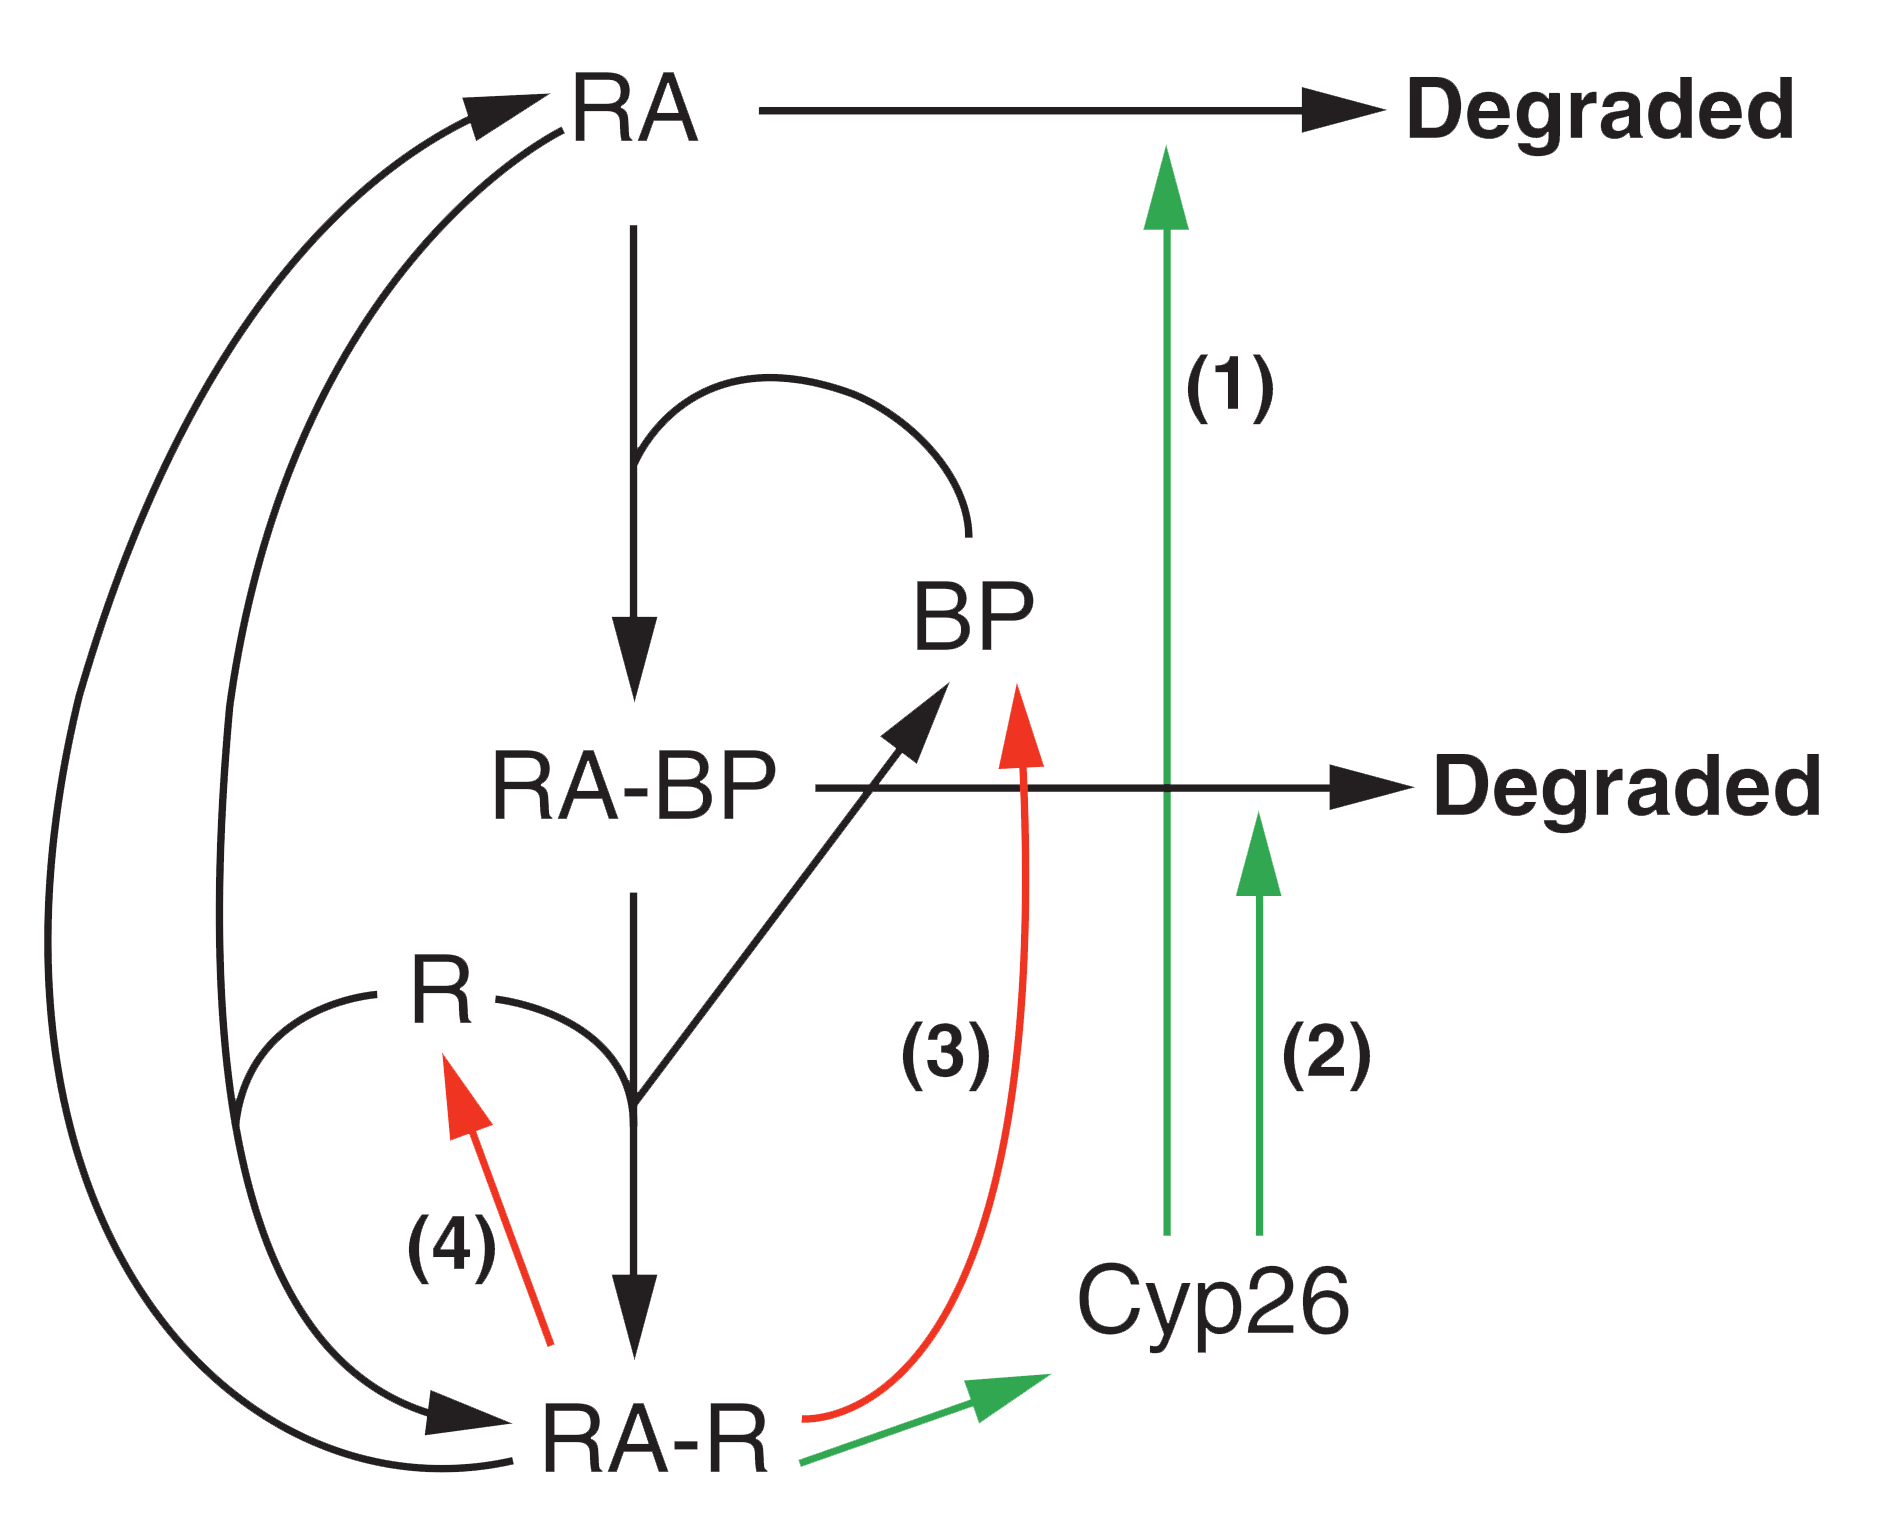
\includegraphics[scale=0.093]{figures/RANetwork.PNG}}
\end{tabular}
